\chapter{Manual de despliegue}

En esta sección se explicará como instalar Spark y ejecutar los ejemplos incluidos en Pyomo con el nuevo módulo \texttt{phspark}.

El primer paso será descargar la distribución de Spark para nuestro sistemas operativo desde la página oficial (\url{http://spark.apache.org/downloads.html}). En el momento de realización de este documento, la última versión es la 2.3.1. Una vez descargado, podemos iniciarlo con la configuración por defecto ejecutando el script \texttt{/sbin/start-all.sh}.

Podemos comprobar que Spark se ha iniciado correctamente accediendo a la interfaz web en \texttt{localhost:8080}, como se ve en la \autoref{fig:manual-spark-web}. En este caso, para acceder al clúster, usaremos la url \texttt{localhost:7077} y esa será la dirección que le indicaremos a Pyomo.\\

\begin{figure}[H]
    \centerline{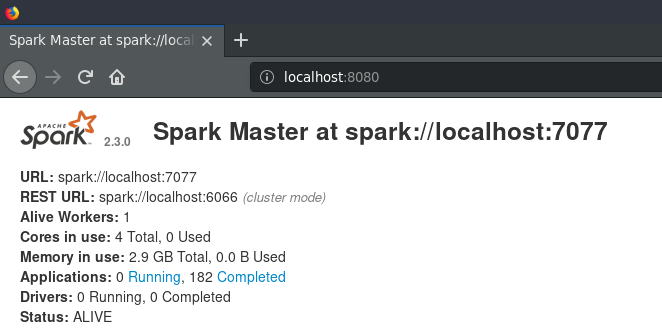
\includegraphics[width=15cm]{figuras/manual/spark-web-interface.png}}
    \caption{Interfaz web de Spark}
    \label{fig:manual-spark-web}
\end{figure}

Teniendo Python 3.6 instalado, vamos a la carpeta raíz del proyecto Pyomo. En esta carpeta hay un archivo \texttt{setup.py}. Para instalar este repositorio de Pyomo como librería en nuestro Python actual, ejecutamos: \\

\texttt{python setup.py develop}. \\

En caso de necesitar librerías adicionales se instalarán usando \texttt{pip}. Algunos requisitos probables son \textit{Pyro} y \textit{Pyutillib}.\\

Con este entorno instalado ya podemos ejecutar los ejemplos de Pyomo utilizando \texttt{phspark}. Para ello, nos movemos a la carpeta \texttt{/pyomo/examples/pysp/farmer} y ejecutamos el siguiente comando:\\

\begin{verbatim}
    runph -r 1 --solver-manager=phspark --traceback --solver=minos
     --solver-io=nl --xhat-method=voting --verbose 
     --model-directory=models/ReferenceModel.py 
     --instance-directory=scenariodata/ScenarioStructure.dat  
     --spark-host=localhost --spark-port=7077
\end{verbatim}

Esto nos mostrará la traza de ejecución y los resultados del problema al final.
